\section{System Overview}
\label{overview}
We present the end-to-end system architecture of \textsc{Mithril} in Figure~\ref{fig:arch}. \textsc{Mitrhil} contains four main components, i.e. policy enforcement module, policy decision module, policy store module, user policy control module. The system sits in between the Apps installed on a user's mobile device and the Android framework. The input to the whole system is a request for data from installed apps on the mobile device. The output of the system is a response containing data or access to a component or an exception stating that the data or component is unavailable. Inside the system the data flows through the policy enforcement module to the policy decision module followed by a request to the policy store and an optional call to the user policy control depending on the request. Further details of the workings of the system's modules is provided in the following sections.

\textsc{Mitrhil}, has two operating modes, i.e. \textsc{Observer} and \textsc{Enforcer}. In the observer mode the system simply stores violation of current policy. After an initial round of data collection and user interaction the system moves to the enforcer mode where it applies the current policy. It keeps on collecting data about any further violations in this mode too, to be intimated to the user in a periodic manner.

%\begin{figure}[tb]
	%\centering
	%\includegraphics[width=\columnwidth]{images/architecture}
	%\caption{System Architecture}
	%\label{fig:arch}
%\end{figure}

\subsection{Definitions: Context, Rule, User-Category, Policy}
\label{defs}
Following are some of the important definitions that we use in this paper to describe the functionality of \textsc{Mithril}.

\begin{definition}
\textsc{Context} has been defined by Dey and Abowd~\cite{Dey99} as: {\em ``[...] any information that can be used to characterize the situation of an entity. An entity is a person, place, or object that is considered relevant to the interaction between a user and application, including the user and applications themselves.''} Dey and Abowd~\cite{Dey99} also decompose context into two categories: \textsc{Primary Context Pieces} (i.e., \textsc{identity, location, activity, time}) and \textsc{Secondary Context Pieces} (pieces of context that are attributes of the primary context pieces for example: a user's phone number can be obtained using the user's identity).
\end{definition}

\begin{definition}
A \textsc{Rule} represented in a logic-based form states the access control \textsc{Action} that will be taken by the system given a certain user \textsc{context}, a requester of data and a requested resource. The three possible actions in our rule are \textsc{Allow, Allow with caveat, Deny}. 
\end{definition}
The ``caveat'' refers to an option whereby the system obfuscates the data returned to the requester. For example we could obfuscate the real location of the user by sharing mock GPS coordinates~\cite{Beresford2011MockDroid}.

\begin{definition}
A \textsc{User-Category} is a classification of a user based on their profession.
\end{definition}

\begin{definition}
A \textsc{Policy}, consists of a set of \textsc{Rules} (also referred to as \textsc{Policy Rules} in this paper), that define access control for data. A policy is applicable to a particular \textsc{User-Category}.
\end{definition}

\subsection{Policy Enforcement}
\label{polenf}
The policy enforcement module is the entry point for our system. It receives as input, data requests from apps and serves them with data as dictated by the ``action'' returned by the policy decision module. In the observer mode, the policy enforcement module does not control any data flow on the mobile device. In this mode it simply passes the data request tuple consisting of the requested component name or type of data and the requester name (henceforth refereed to as: request meta-data) to the policy decision module. In the enforcer mode, it passes on the request meta-data but expects the policy decision module to provide an ``action''. If the action is to allow data flow, it simply makes a request to the Android framework for the data and returns the same to the requesting app. If the action is to deny the data flow, it prohibits the request from going any further. If the action is to ``allow with caveat'' then the data is obtained from the Android framework and a data obfuscation sub-module modifies the data before passing it on to the requesting app. Obfuscation could be done by faking location information~\cite{Beresford2011MockDroid} or other data from the Android framework.

\subsection{Policy Decision}
\label{poldec}
The policy decision module receives as input, the request meta-data from the policy enforcement module. The current context is obtained using a context synthesizer sub-module. The context synthesizer keeps updated user context facts obtained from a reasoner using ontologies to infer associations between sensor data and user context. A similar technique for context inference from low level sensor information was explored in~\cite{gu2004ontology}. We use the Platys ontology~\cite{Jagtap2011Privacy} to semantically represent user context and app meta-data. We use classes defined in the Platys ontology to define hierarchical context models that enables us to generalize or specialize over primary and secondary user context pieces. An example of how this is used is shown in section~\ref{policyControl}.

We use a knowledge-base on the phone that stores facts about apps including app categories. The facts are extracted from various sources like the Android Marketplace~\footnote{Android Market Place:~\url{http://goo.gl/4GHoFo}} and the DBpedia ontology~\cite{mendes2012dbpedia}. The facts include meta-data like app manufacturer, download count, maturity rating, user rating, developer country of origin, number and types of permissions requested by the app etc. The facts about the user context and apps are stored in form of RDF triples, which help us query the knowledge-base for properties like app types or location types. These information enables the inference mechanism as the rules are stated in terms of the type properties of apps and user context.

\begin{figure}[tb]
	\centering
	\includegraphics[width=\columnwidth]{images/architecture}
	\caption{System Architecture}
	\label{fig:arch}
\end{figure}

The final piece of information needed to make a decision are the rules for the current request meta-data, which are provided by the policy storage module. A requester, resource tuple can have multiple policy rules applicable based on contextual conditions. Once the rules are obtained, using the context and app facts from the knowledge-base a specific rule applicable is inferred by an OWL-DL reasoner. The consequent of the chosen rule is the applicable action. If the action is deny or allow with caveat, then the data request is marked as a possible violation of current policy rules. 

In the observer mode, the violation meta-data, which consists of the request meta-data along-with the applicable rule and user context is forwarded to the User Policy Control module and no response is sent to the policy enforcement module. In the enforcer mode however, the action inferred by the reasoner is returned to the policy enforcement module and at the same time the violation meta-data is forwarded to the User Policy Control module.

\subsection{Policy Store}
\label{polsto}
The policy storage module has a database containing the currently applicable policy for the user-category of the mobile device's user. The user chooses an applicable user-category, when the system starts for the first time and the default for said category is then downloaded on the mobile device. The storage module receives as input a requester app information and information about the requested resource. It searches the policy database for the applicable policy rules and returns the same to the policy decision module. The second task that the policy storage handles is updating a policy rule as requested by the user policy control module. Let us take a look at how rules are represented in \textsc{Mithril}. 

\subsubsection{Rule Representation}
\label{ruleRepresentation}
Rules, in our system, are represented using the Semantic Web Rule Language (SWRL)~\cite{horrocks2004swrl}. Rules are composed of antecedents which define the context in which a certain rule is applicable, the requesting entity and the requested resource. The consequent of a rule defines the action to be taken. Following is an example rule where, we have an app that belongs to the social media category. We are taking a look at a rule from the policy for a graduate student. The rule states that while the student is in her university building, social media apps are not allowed to access the camera on her mobile device. We call this rule \textsc{SocialMediaCameraAccessRule} and can be seen in Figure~\ref{ruleSimple}. The policy is called \textsc{GradStudentPolicy}. Given all of above assumptions, we represent the afore-mentioned SocialMediaCameraAccessRule as:-

\begin{figure}[tb]
	\centering
	\noindent\fbox{
		\parbox{0.95\columnwidth}{
			$resourceRequested\left(?r, Camera\right) \wedge\\requestingApp\left(?app\right) \wedge\\hasAppType\left(?app, SocialMedia\right)\wedge\\User\left(?u\right) \wedge\\userLocation\left(?u, ?l\right) \wedge\\hasLocationType\left(?l, University Building\right)\\\rightarrow\\AccessLevel\left(Deny\right)$
		}
	}
	\caption{Simple rule for controlling social media camera access}
	\label{ruleSimple}
\end{figure}

We can have a more detailed version of the same rule with more conditions incorporated. The resultant rule would be more complex but would give higher degree of granularity with respect to their privacy and security policy rules. The more granular second rule could be stated as ``do not allow camera access to SocialMedia apps when the time of day is between 9AM and 5PM and it is a weekday and the user is at university building location in presence of his advisor and has a meeting scheduled with her advisor''. We can see this rule in Figure~\ref{ruleLong}.
\begin{figure}[tb]
	\centering
	\noindent\fbox{
		\parbox{0.95\columnwidth}{
			$resourceRequested\left(?r, Camera\right) \wedge\\requestingApp\left(?app\right) \wedge\\hasAppType\left(?app, SocialMedia\right)\wedge\\User\left(?u\right) \wedge\\userTime\left(?u, ?t\right) \wedge\\timeAfter\left(?t, 0900\right) \wedge\\timeBefore\left(?t, 1700\right) \wedge\\userDayOfWeek\left(?u, ?d\right) \wedge\\hasDayType\left(?d, weekday\right) \wedge\\userActivity\left(?a\right) \wedge\\hasActivityType\left(?a, Advisor\_Meeting\right) \wedge\\userpresenceInfo\left(?p\right) \wedge\\hasPresenceType\left(?p, Advisor\right)\wedge\\userLocation\left(?u, ?l\right) \wedge\\hasLocationType\left(?l, University Building\right)\\\rightarrow\\AccessLevel\left(Deny\right)$
		}
	}
	\caption{Rule with higher granularity, for controlling social media camera access}
	\label{ruleLong}
\end{figure}